\documentclass[aspectratio=169]{beamer}

\usetheme{Madrid}
\setbeamertemplate{navigation symbols}{}

\definecolor{fptOrange}{HTML}{F37021}
\definecolor{fptNavy}{HTML}{1A2B4A}
\definecolor{fptLight}{HTML}{FFF5EE}
\definecolor{positive}{HTML}{0173B2}
\definecolor{negative}{HTML}{DE8F05}
\definecolor{emphasis}{HTML}{029E73}
\definecolor{neutral}{gray}{0.55}
\definecolor{cbPurple}{HTML}{CC78BC}

\setbeamercolor{palette primary}{bg=fptNavy,fg=white}
\setbeamercolor{palette secondary}{bg=fptNavy!80,fg=white}
\setbeamercolor{palette tertiary}{bg=fptOrange,fg=white}
\setbeamercolor{palette quaternary}{bg=fptNavy,fg=white}
\setbeamercolor{structure}{fg=fptOrange}
\setbeamercolor{frametitle}{bg=fptNavy,fg=white}
\setbeamercolor{title}{bg=fptNavy,fg=white}
\setbeamercolor{subtitle}{fg=fptOrange}
\setbeamercolor{section in toc}{fg=fptNavy}
\setbeamercolor{normal text}{fg=fptNavy}
\setbeamercolor{block title}{bg=fptNavy!10,fg=fptNavy}
\setbeamercolor{block body}{bg=fptNavy!4,fg=fptNavy}
\setbeamercolor{block title alerted}{bg=fptOrange!20,fg=fptOrange!80!black}
\setbeamercolor{block body alerted}{bg=fptOrange!6,fg=fptNavy}
\setbeamercolor{block title example}{bg=emphasis!15,fg=emphasis!70!black}
\setbeamercolor{block body example}{bg=emphasis!4,fg=fptNavy}

\usepackage{fontspec}
\setbeamerfont{title}{size=\Large,series=\bfseries}
\setbeamerfont{subtitle}{size=\normalsize,series=\normalfont}
\setbeamerfont{frametitle}{size=\large,series=\bfseries}
\setbeamerfont{block title}{size=\normalsize,series=\bfseries}

\usepackage{amsmath,amssymb,booktabs,array}
\usepackage{graphicx}
\usepackage{tikz}
\usetikzlibrary{arrows.meta,positioning,shapes.geometric,automata}
\usepackage{eso-pic}

\setbeamertemplate{headline}{}

\setbeamertemplate{frametitle}{%
  \nointerlineskip%
  \begin{beamercolorbox}[wd=\paperwidth,ht=1.1cm,dp=0.2cm,leftskip=8pt,rightskip=8pt]{frametitle}%
    \usebeamerfont{frametitle}\color{white}\insertframetitle%
    \hfill%
    
\includegraphics[height=0.88cm]{../../docs/logo/fpt_logo.png}%
  \end{beamercolorbox}%
  \begin{beamercolorbox}[wd=\paperwidth,ht=2pt,dp=0pt]{palette tertiary}%
  \end{beamercolorbox}%
}

\setbeamertemplate{footline}{%
  \leavevmode%
  \begin{beamercolorbox}[wd=\paperwidth,ht=2.5ex,dp=1.2ex,leftskip=8pt,rightskip=8pt]{palette primary}%
    \usebeamerfont{footline}\footnotesize
    \insertshortauthor\hfill
    \insertshorttitle\hfill
    \insertframenumber\,/\,\inserttotalframenumber\hspace{4pt}
  \end{beamercolorbox}%
}

\newcommand{\pos}[1]{\textcolor{positive}{#1}}
\newcommand{\con}[1]{\textcolor{negative}{#1}}
\newcommand{\HL}[1]{\textcolor{emphasis}{#1}}
\newcommand{\good}[1]{\textcolor{emphasis}{\textbf{#1}}}
\newcommand{\best}[1]{\textcolor{fptOrange}{\textbf{#1}}}

\title[Vietnamese GraphRAG --- Review 3]{A Study and Evaluation of Graph RAG on Wikipedia Data}
\subtitle{Vietnamese Multi-hop Question Answering over Wikipedia}
\author[Trung, Anh, Khoi]{Huynh Quoc Trung (QE180038) \and Nhu Quang Anh (QE180005) \and Pham Ngo Dinh Khoi (QE180110)}
\institute{FPT University\\[4pt]\small\textit{Supervisors:} Lê Trung Hiếu \quad Đặng Nguyên Bình}
\date{Gia Lai, August 7, 2026}

\begin{document}

\begin{frame}[plain]
  \centering
  
\includegraphics[height=1.25cm]{../../docs/logo/fpt_logo.png}\par\vspace{0.4cm}
  \titlepage
  \vfill
  \small Project period: May 1, 2026 -- August 7, 2026
\end{frame}

\begin{frame}{Table of Contents}
\begin{columns}[T]
\column{0.48\textwidth}
\begin{enumerate}
  \item Problem, Scope, and Objectives
  \item Users and Innovation
  \item System Architecture
  \item Dataset and Data Pipeline
  \item Ingestion and Neo4j Graph
  \item Retrieval Design
\end{enumerate}
\column{0.48\textwidth}
\begin{enumerate}
  \setcounter{enumi}{6}
  \item Evaluation and Results
  \item Limitations
  \item Contributions and Conclusion
\end{enumerate}
\end{columns}
\end{frame}

\begin{frame}{Research Problem and Objectives}
\begin{block}{Problem}
Vietnamese multi-hop QA needs complete, traceable evidence across Wikipedia pages. Text-only retrieval can miss the relation connecting the required facts.
\end{block}
\begin{enumerate}
  \item Build a reproducible Vietnamese Wikipedia corpus with stable evidence IDs.
  \item Combine lexical, dense, graph, and community retrieval in Neo4j.
  \item Evaluate answer, supporting evidence, abstention, latency, and ablations.
\end{enumerate}
\end{frame}

\begin{frame}{Users, Applicability, and Innovation}
\begin{columns}[T]
\column{.5\textwidth}
\begin{block}{Real users and value}
\begin{itemize}
\item Students and researchers need faster evidence synthesis across multiple Wikipedia pages.
\item Journalists and analysts need verifiable Vietnamese citations rather than answer-only summaries.
\item AI developers can reuse the corpus, graph schema, and evaluation pipeline.
\end{itemize}
\end{block}
\column{.5\textwidth}
\begin{block}{What is new in our system}
\begin{itemize}
\item Local-first Vietnamese GraphRAG with auditable evidence IDs.
\item WRRF combines lexical, vector, graph, and community retrieval signals.
\item ViWikiHop adds answerable and unanswerable multi-hop items with quality control.
\end{itemize}
\end{block}
\end{columns}
\end{frame}

\begin{frame}{System Architecture}
\begin{center}
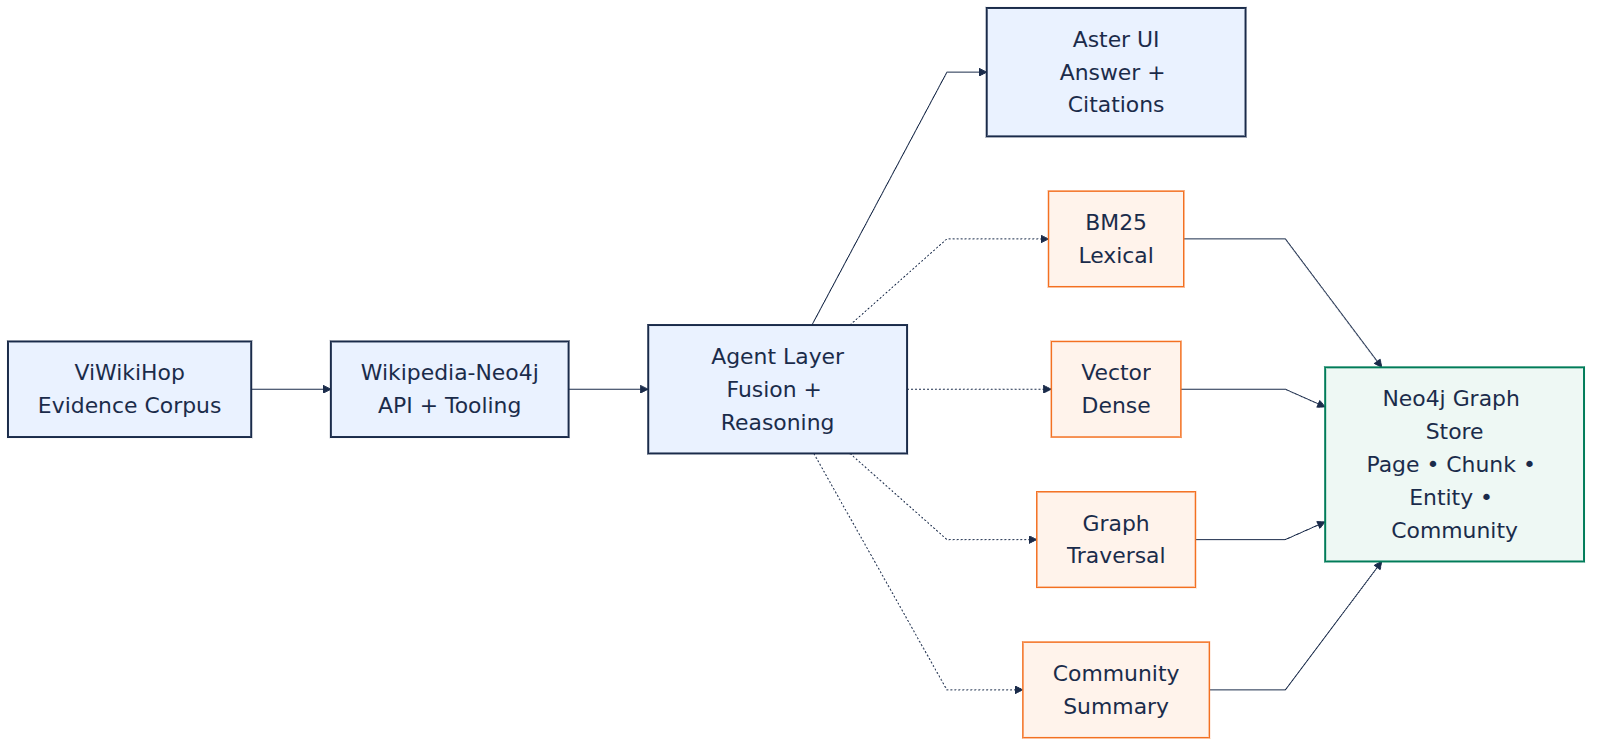
\includegraphics[width=0.96\textwidth,height=0.69\textheight,keepaspectratio]{rendered/system-architecture.png}
\end{center}
\vspace{2pt}
{\scriptsize ViWikiHop controls corpus evidence, Wikipedia-Neo4j performs retrieval and reasoning, and Aster presents the live QA interface.}
\end{frame}

\begin{frame}[shrink=5]{Dataset Motivation}
\begin{tabular}{lccc}
\toprule
Dataset & Size & Role & Stage \\
\midrule
Vietnamese Wikipedia (final corpus) & $\sim$590K pages & Corpus and graph construction & R1--R3 \\
UIT-ViQuAD 2.0 & 36,457 QA pairs & Retrieval benchmark & R1--R2 \\
ViWikiHop & 1,600 QA items & Multi-hop end-to-end evaluation & R2--R3 \\
\bottomrule
\end{tabular}
\vspace{.35cm}
\begin{itemize}
\item Review 1 focused on feasibility: identify real Vietnamese sources and measurable benchmarks.
\item Review 2 and Review 3 converted that plan into a grouped, answerable/unanswerable test set for GraphRAG evaluation.
\end{itemize}
\end{frame}

\begin{frame}[shrink=15]{Data Pipeline --- Corpus Filtering}
\begin{columns}[T]
\column{0.52\textwidth}
\begin{block}{11-Stage Filter: \texttt{viwiki-20260501} Snapshot}
\begin{tabular}{@{}lrr@{}}
\toprule
\textbf{Stage} & \textbf{Count} & \textbf{Drop} \\
\midrule
Initial dump        & 1{,}614{,}015 & --- \\
Redirect filter     & 1{,}300{,}130 & $-$313K \\
Disambiguation      & 1{,}284{,}671 & $-$15K \\
List pages          & 1{,}279{,}292 & $-$5K \\
Year/date pages     & 1{,}276{,}304 & $-$3K \\
Dup-line filter     & 1{,}275{,}171 & $-$1K \\
Word count pre      &   414{,}397 & $-$861K \\
Orphan filter       &   397{,}438 & $-$17K \\
Word count final    &   357{,}747 & $-$40K \\
Stop words          &   357{,}736 & $-$11 \\
Exact dedup         &   357{,}714 & $-$22 \\
\textbf{MinHash dedup} & \textbf{353{,}498} & $-$4K \\
\bottomrule
\end{tabular}
\end{block}

\column{0.44\textwidth}
\begin{exampleblock}{Key Design Choices}
\begin{itemize}\scriptsize\setlength\itemsep{2pt}
  \item Word count pre-filter: largest single drop ($-$861K stubs)
  \item Orphan filter: removes unlinked articles ($-$17K)
  \item MinHash dedup: Jaccard $\geq 0.85$ threshold
  \item \textbf{No} punctuation-ratio filter: Wikipedia tables/lists naturally break the 60\% threshold; dropped after analysis
\end{itemize}
\end{exampleblock}

\begin{block}{Result}
{\small $1{,}614{,}015 \rightarrow$ \pos{\textbf{353{,}498}} articles\\
(21.9\% of original dump retained)\\
Snapshot: \texttt{viwiki-20260501}}
\end{block}
\end{columns}
\vspace{2pt}
{\scriptsize This slide reports the Review 2 filtering experiment snapshot; later production ingestion uses a different cleaned corpus snapshot.}
\end{frame}

\begin{frame}{Corpus Construction}
\small
\centering
\begin{block}{Final production corpus used in the current system}
\begin{tabular}{lrrr}
\toprule
Stage & Retained pages & Removed & Retention \\
\midrule
Input snapshot & 1,288,472 & -- & 100.00\% \\
Structural filters & 884,219 & 404,253 & 68.63\% \\
Quality filters & 641,738 & 242,481 & 49.81\% \\
Orphan filter & 598,314 & 43,424 & 46.44\% \\
Deduplication & \best{589,742} & 8,572 & \best{45.77\%} \\
\bottomrule
\end{tabular}
\end{block}
\vspace{.45cm}
\begin{itemize}
\item Removes redirects, lists, weak Vietnamese pages, duplicates, and graph orphans.
\item Retains cleaned text, wikilinks, provenance, and stable article-local segment IDs for downstream ingestion.
\end{itemize}
\end{frame}

\begin{frame}[shrink=20]{Data Pipeline --- ViWikiHop Schema v0.4}
\begin{columns}[T]
\column{0.50\textwidth}
\begin{block}{Entry Schema (schema v0.4)}
{\scriptsize
\begin{tabular}{@{}lp{3.2cm}@{}}
\toprule
\textbf{Field} & \textbf{Description} \\
\midrule
\texttt{\_id}           & \texttt{hw-} / \texttt{syn-mh-} / \texttt{uvq-} \\
\texttt{question}       & Vietnamese question \\
\texttt{answer}         & Empty if unanswerable \\
\texttt{supporting\_facts} & Evidence refs \\
\texttt{context}        & Paragraph segments \\
\texttt{type}           & 8 reasoning types \\
\texttt{level}          & easy / medium / hard \\
\texttt{source}         & 3 sources \\
\texttt{num\_hops}      & $\geq 1$ \\
\texttt{is\_vi\_exclusive} & VI-exclusive track \\
\texttt{is\_impossible} & Unanswerable flag \\
\texttt{decomposition}  & Sub-Q/A per hop \\
\texttt{plausible\_answer} & For unanswerable only \\
\bottomrule
\end{tabular}
}
\end{block}

\column{0.46\textwidth}
\begin{block}{3 Data Sources}
\begin{tabular}{@{}ll@{}}
\toprule
\textbf{Source} & \textbf{Description} \\
\midrule
\texttt{hw-}      & Human annotated \\
\texttt{syn-mh-}  & KG walk synthesis \\
\texttt{uvq-}     & ViQuAD 2.0 import \\
\bottomrule
\end{tabular}
\end{block}

\begin{alertblock}{Schema v0.4 Key Invariants}
\begin{itemize}\scriptsize\setlength\itemsep{2pt}
  \item Single-hop: \texttt{decomposition} = $[\,]$
  \item Unanswerable: \texttt{answer}=\texttt{""}, non-empty \texttt{plausible\_answer}
  \item Multi-hop: $|\texttt{decomposition}|$ = \texttt{num\_hops}
  \item UIT-ViQuAD: \texttt{is\_vi\_exclusive} always false
\end{itemize}
\end{alertblock}
\end{columns}
\end{frame}

\begin{frame}[shrink=15]{Data Pipeline --- Reasoning Types \& Difficulty}
\begin{columns}[T]
\column{0.50\textwidth}
\begin{block}{8 Reasoning Types}
\begin{tabular}{@{}lp{3.5cm}@{}}
\toprule
\textbf{Type} & \textbf{Description} \\
\midrule
\texttt{lookup}        & One article, one fact \\
\texttt{bridge}        & A $\to$ bridge entity $\to$ B \\
\texttt{comparison}    & Compare $\geq 2$ article values \\
\texttt{intersection}  & Entity from $\geq 2$ constraints \\
\texttt{temporal}      & Date order / chronology \\
\texttt{numerical}     & Arithmetic or counting \\
\texttt{fan-out}       & Aggregate related entities \\
\texttt{unanswerable}  & No valid answer in context \\
\bottomrule
\end{tabular}
\end{block}

\column{0.46\textwidth}
\begin{block}{3-D Difficulty Rubric}
{\small Score = hop\_count + lexical\_overlap + reasoning\_op}\\[4pt]
\begin{tabular}{@{}lccc@{}}
\toprule
\textbf{Score} & \textbf{Hop} & \textbf{Lexical} & \textbf{ReasonOp} \\
\midrule
0 & 1-hop     & $\geq 60\%$ & lookup \\
1 & 2-hop     & 30--60\%    & bridge/comparison \\
2 & $\geq$3-hop & $< 30\%$ & temporal/numerical/\ldots \\
\bottomrule
\end{tabular}

\vspace{4pt}
\begin{tabular}{@{}ll@{}}
\toprule
\textbf{Total (0--6)} & \textbf{Level} \\
\midrule
0--1 & \HL{easy} \\
2--3 & \con{medium} \\
4--6 & \pos{hard} \\
\bottomrule
\end{tabular}
\end{block}
\end{columns}
\end{frame}

\begin{frame}[shrink=10]{Data Pipeline --- QA Generation \& QC}
\begin{columns}[T]
\column{0.50\textwidth}
\begin{block}{QA Generation Pipeline}
\begin{enumerate}\small\setlength\itemsep{3pt}
  \item \textbf{Bridge Extraction} --- follow \texttt{[[wikilinks]]} to build article-pair bridges; no Neo4j walk
  \item \textbf{LLM Sampling} --- prompt LLM to generate questions directly from bridge pairs (no templates)
  \item \textbf{Labelling} --- \textbf{Gemini 2.5 Flash Lite} reads difficulty rubric and assigns type + level
  \item \textbf{Verification} --- \textbf{DeepSeek V3 Pro} independently verifies label and answer grounding
\end{enumerate}
\end{block}

\begin{exampleblock}{Sample Entry ID}
{\scriptsize \texttt{syn-mh-viex-b1-a-00001}\\
type=bridge, level=medium, num\_hops=2\\
is\_vi\_exclusive=true, source=synthetic-multihop}
\end{exampleblock}

\column{0.46\textwidth}
\begin{block}{Two-Model QC Gate}
\begin{tabular}{@{}lp{2.8cm}@{}}
\toprule
\textbf{Model} & \textbf{Role} \\
\midrule
Gemini 2.5 Flash Lite & Label (type, level, decomposition) \\
DeepSeek V3 Pro       & Verify label + grounding \\
\bottomrule
\end{tabular}
\smallskip

{\scriptsize Gate logic: entry passes only when both models agree on answer grounding; label is taken from Gemini, rejected if DeepSeek flags a mismatch.}
\end{block}

\begin{block}{Schema QC (post-gate)}
\begin{itemize}\scriptsize\setlength\itemsep{1pt}
  \item Well-formedness: non-empty fields, schema v0.4
  \item Grounding: answer in supporting\_facts verbatim
  \item Natural phrasing: no \textit{``Theo bài viết''} phrases
  \item Dedup: exact + MinHash ($J \geq 0.85$)
\end{itemize}
\end{block}
\end{columns}
\end{frame}

\begin{frame}[shrink=4]{ViWikiHop Dataset and Quality Controls}
\small
\begin{columns}[T]
\column{.50\textwidth}
\begin{tabular}{lrrr}
\toprule
Split & Answerable & Unanswerable & Total \\
\midrule
Train & 783 & 337 & 1,120 \\
Development & 168 & 72 & 240 \\
Test & 167 & 73 & 240 \\
\midrule
Total & 1,118 & 482 & 1,600 \\
\bottomrule
\end{tabular}
\column{.46\textwidth}
\begin{block}{Quality controls}
\begin{itemize}
\item Group-aware split to reduce leakage across related questions.
\item Includes both answerable and unanswerable items for abstention testing.
\item Manual review and schema checks after automatic generation.
\end{itemize}
\end{block}
\end{columns}
\end{frame}

\begin{frame}[shrink=5]{AI Pipeline --- Data Ingestion}
\vspace{6pt}
\centering
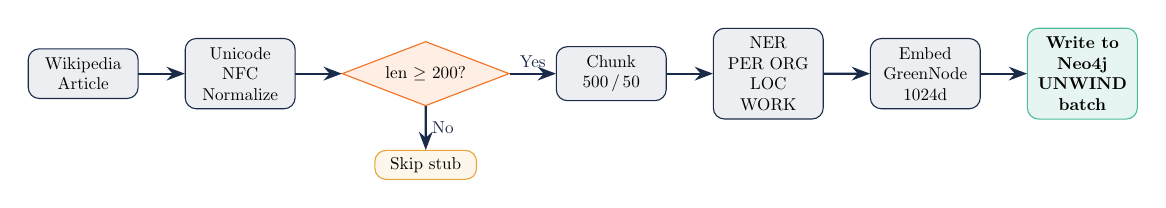
\begin{tikzpicture}[scale=0.62, transform shape,
  node distance=0.45cm and 0.95cm,
  box/.style={draw=fptNavy, fill=fptNavy!8, rounded corners=4pt,
              font=\normalsize, text width=1.9cm, align=center,
              inner sep=5pt, minimum height=0.75cm},
  dec/.style={draw=fptOrange, fill=fptOrange!12, diamond, aspect=2.6,
              font=\normalsize, align=center, inner sep=4pt},
  skip/.style={draw=negative!80, fill=negative!8, rounded corners=4pt,
               font=\normalsize, text width=1.8cm, align=center, inner sep=4pt},
  db/.style={draw=emphasis!70, fill=emphasis!10, rounded corners=4pt,
             font=\normalsize\bfseries, text width=1.9cm, align=center, inner sep=5pt},
  arr/.style={-Stealth, fptNavy, thick}
]
\node[box] (wiki)                    {Wikipedia Article};
\node[box, right=of wiki]  (norm)    {Unicode NFC Normalize};
\node[dec, right=of norm]  (len)     {len $\geq$ 200?};
\node[skip, below=0.9cm of len] (skip) {Skip stub};
\node[box, right=of len]   (chunk)   {Chunk\\500\,/\,50};
\node[box, right=of chunk] (ner)     {NER\\PER ORG\\LOC WORK};
\node[box, right=of ner]   (embed)   {Embed\\GreenNode\\1024d};
\node[db,  right=of embed] (neo4j)   {Write to Neo4j\\UNWIND batch};
\draw[arr] (wiki)  -- (norm);
\draw[arr] (norm)  -- (len);
\draw[arr] (len)   -- node[above, font=\normalsize]{Yes} (chunk);
\draw[arr] (len)   -- node[right, font=\normalsize]{No}  (skip);
\draw[arr] (chunk) -- (ner);
\draw[arr] (ner)   -- (embed);
\draw[arr] (embed) -- (neo4j);
\end{tikzpicture}

\vspace{8pt}
{\small
\begin{tabular}{@{}lll@{}}
\toprule
\textbf{Stub filter} & \textbf{NER backend} & \textbf{Embedding} \\
\midrule
1.29M $\to$ $\sim$590K cleaned articles & \texttt{wikilink} (Typed F1 = 46.9\%) & GreenNode 1024-dim \\
\bottomrule
\end{tabular}}
\end{frame}

\begin{frame}{Knowledge Graph and Retrieval}
\begin{center}
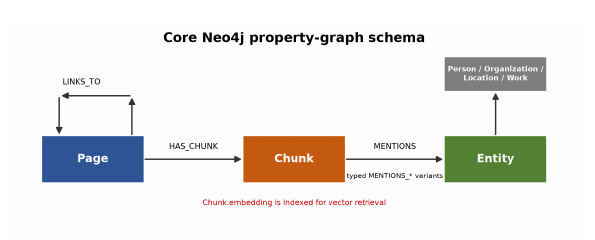
\includegraphics[width=0.84\textwidth,height=0.53\textheight,keepaspectratio]{rendered/fig_02_graph_schema.png}
\end{center}
\vspace{.15cm}
\begin{itemize}
\item Nodes: \texttt{Page}, \texttt{Chunk}, typed \texttt{Entity}, and \texttt{Community}; edges preserve mentions and article links.
\item Four retrieval channels: BM25, dense vectors, entity graph, and community summaries.
\end{itemize}
\end{frame}

\begin{frame}[shrink=4]{Neo4j Ingestion Status}
\begin{block}{Retrieval-ready graph}
\centering
\begin{tabular}{lrl}
\toprule
Metric & Value & Notes \\
\midrule
Pages & 2,339 & articles indexed in current Neo4j snapshot \\
Chunks & 31,470 & segmented evidence units in that snapshot \\
Entities & 22,736 & total entity nodes \\
\texttt{MENTIONS} & 136,080 & chunk-to-entity links \\
\texttt{LINKS\_TO} & 4,956 & page-to-page links \\
Communities & 46 & clustered summaries \\
Chunk embeddings & 31,470 / 31,470 & 100\% coverage \\
Typed entities & 20,560 / 22,736 & \(\sim\)90.4\% typed coverage \\
Generic entities remaining & 2,241 & untyped tail after extraction \\
\bottomrule
\end{tabular}
\end{block}
\vspace{2pt}
{\scriptsize This graph is the retrieval snapshot used for the reported experiments, not the full cleaned Wikipedia corpus.}
\end{frame}

\begin{frame}[shrink=5]{Neo4j Backbone --- Page to Chunk}
\begin{columns}[T]
\column{0.55\textwidth}
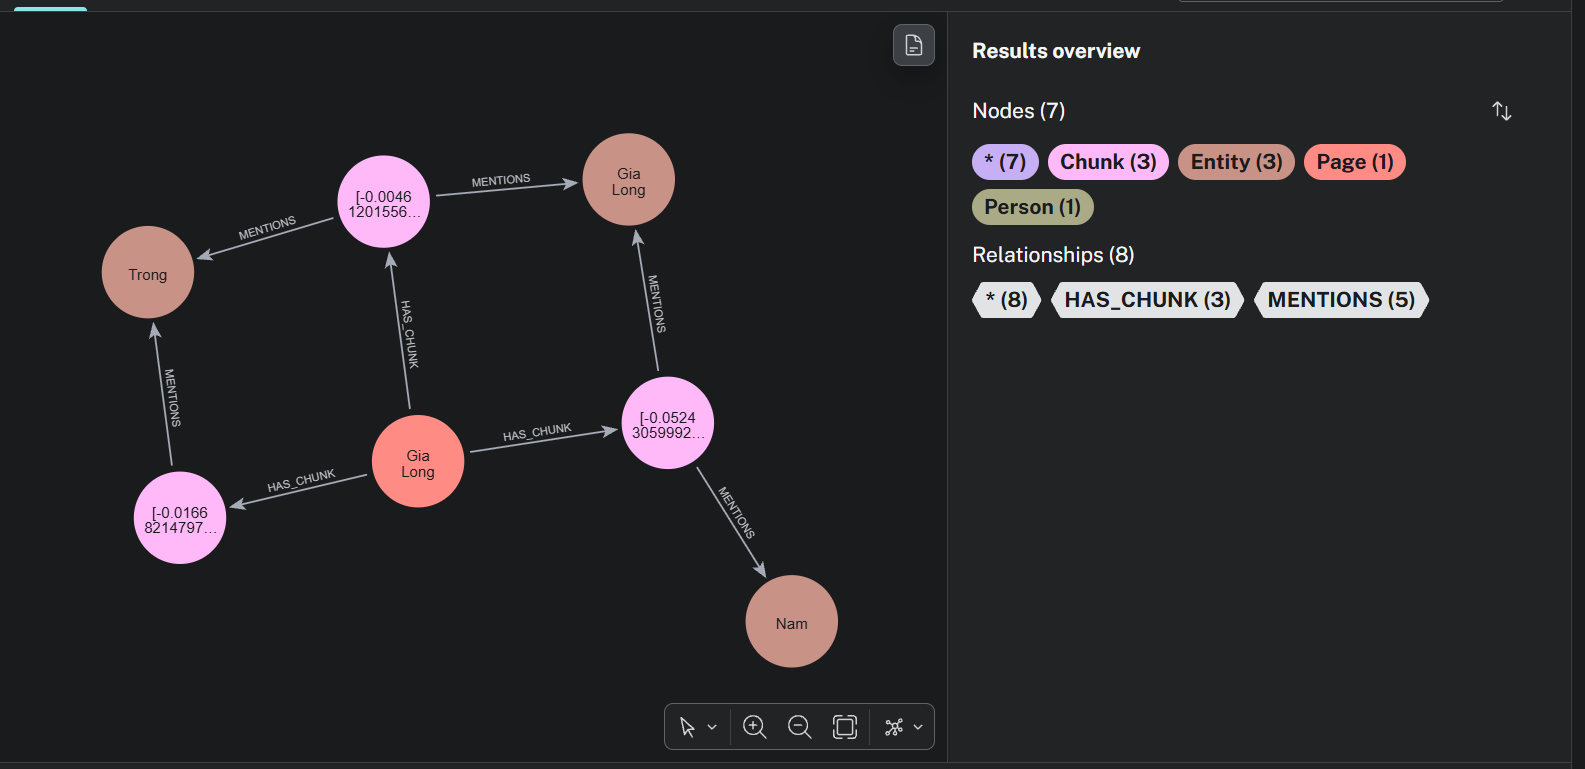
\includegraphics[width=\textwidth,height=0.62\textheight,keepaspectratio]{neo4j-screen/anh1.png}
\column{0.39\textwidth}
\begin{block}{Graph backbone}
\begin{itemize}
\item \texttt{Page -[:HAS\_CHUNK]-> Chunk}
\item Pages preserve article-level provenance while chunks keep retrieval at evidence granularity.
\item This backbone ties every evidence unit to its source document.
\end{itemize}
\end{block}
\end{columns}
\end{frame}

\begin{frame}[shrink=5]{Neo4j Backbone --- Chunk to Entity}
\begin{columns}[T]
\column{0.55\textwidth}
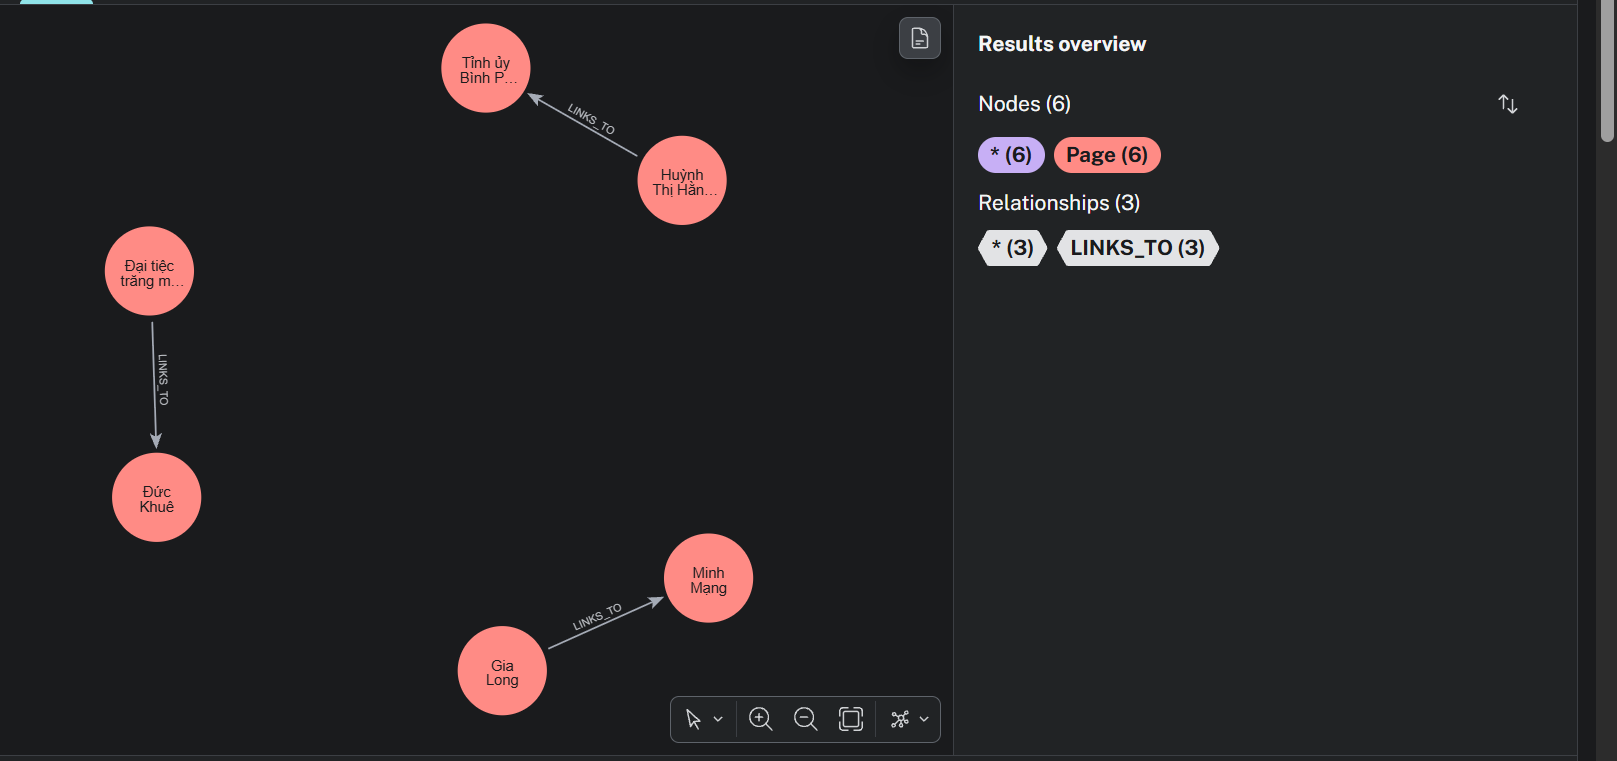
\includegraphics[width=\textwidth,height=0.62\textheight,keepaspectratio]{neo4j-screen/anh2.png}
\column{0.39\textwidth}
\begin{block}{Document and entity layer}
\begin{itemize}
\item \texttt{Page -[:LINKS\_TO]-> Page}
\item Typed entities include \texttt{Person}, \texttt{Organization}, and \texttt{Work}.
\item This layer preserves article navigation and semantic typing together.
\end{itemize}
\end{block}
\end{columns}
\end{frame}

\begin{frame}[shrink=5]{Neo4j Backbone --- Page Links and Typed Entities}
\begin{columns}[T]
\column{0.55\textwidth}
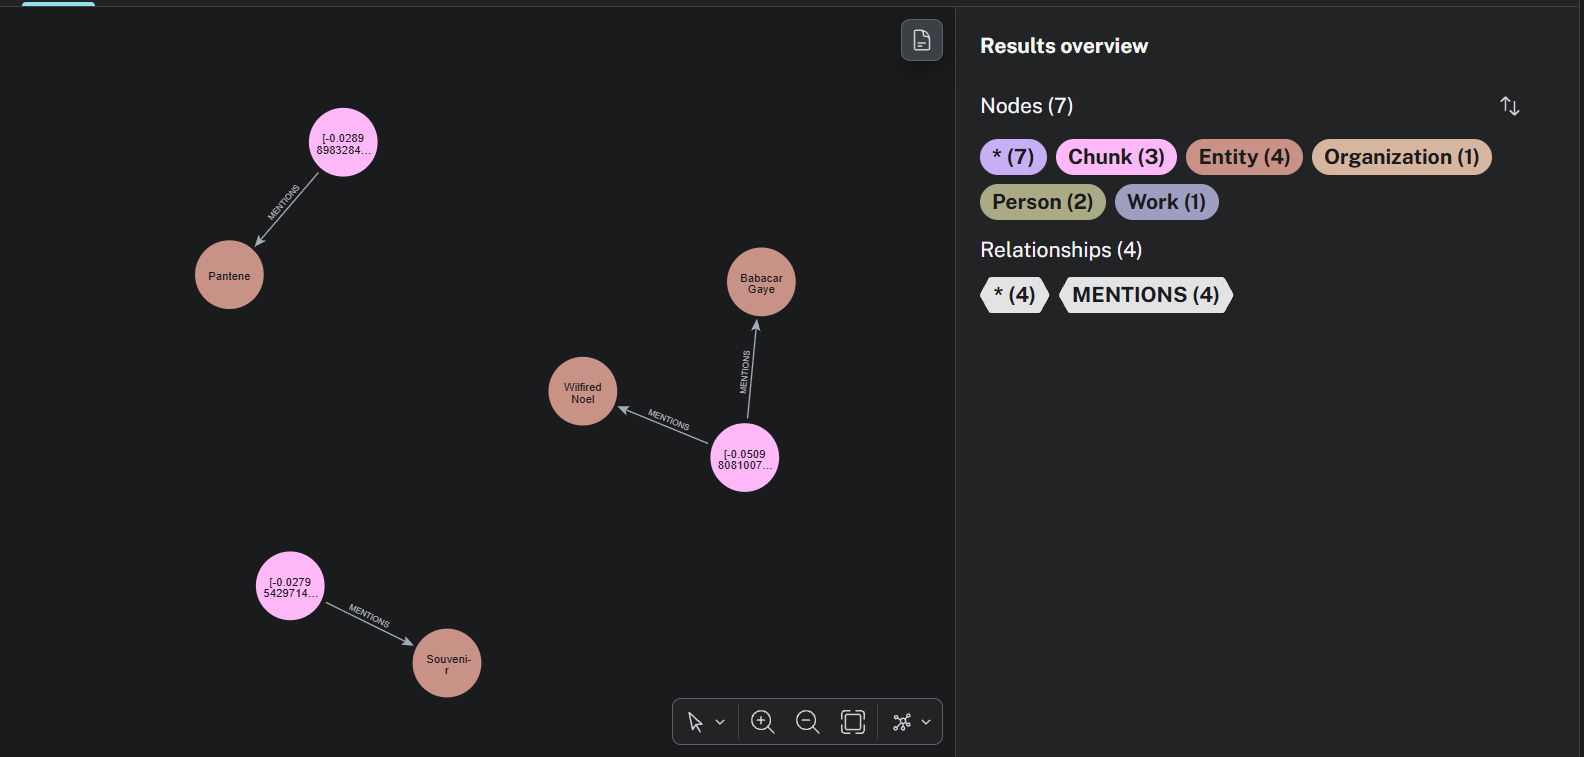
\includegraphics[width=\textwidth,height=0.62\textheight,keepaspectratio]{neo4j-screen/anh3.png}
\column{0.39\textwidth}
\begin{block}{Mention structure}
\begin{itemize}
\item \texttt{Chunk -[:MENTIONS]-> Entity}
\item Entity nodes support graph traversal beyond raw text retrieval.
\item Mentions connect evidence chunks to reusable semantic nodes.
\end{itemize}
\end{block}
\end{columns}
\end{frame}

\begin{frame}[shrink=5]{Neo4j Semantic Relations --- Entity Layer}
\begin{columns}[T]
\column{0.55\textwidth}
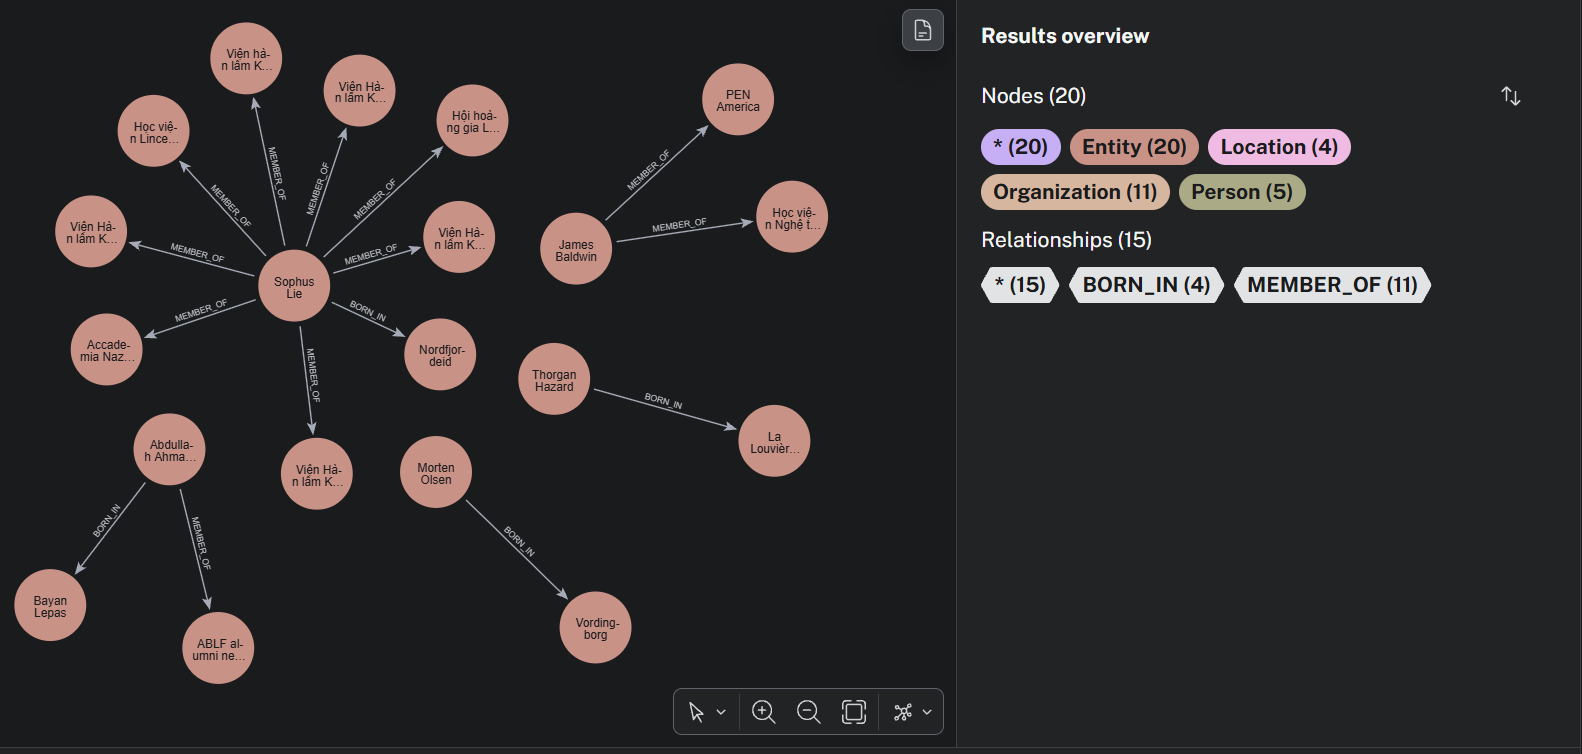
\includegraphics[width=\textwidth,height=0.62\textheight,keepaspectratio]{neo4j-screen/anh5.png}
\column{0.39\textwidth}
\begin{block}{Semantic layer}
\begin{itemize}
\item \texttt{Entity -[:BORN\_IN|MEMBER\_OF]-> Entity}
\item Higher-level relations support multi-hop evidence chains.
\item Retrieval can move from mentions to semantic relations when text alone is insufficient.
\end{itemize}
\end{block}
\end{columns}
\end{frame}

\begin{frame}[shrink=5]{Neo4j Semantic Relations --- Community Layer}
\begin{columns}[T]
\column{0.55\textwidth}
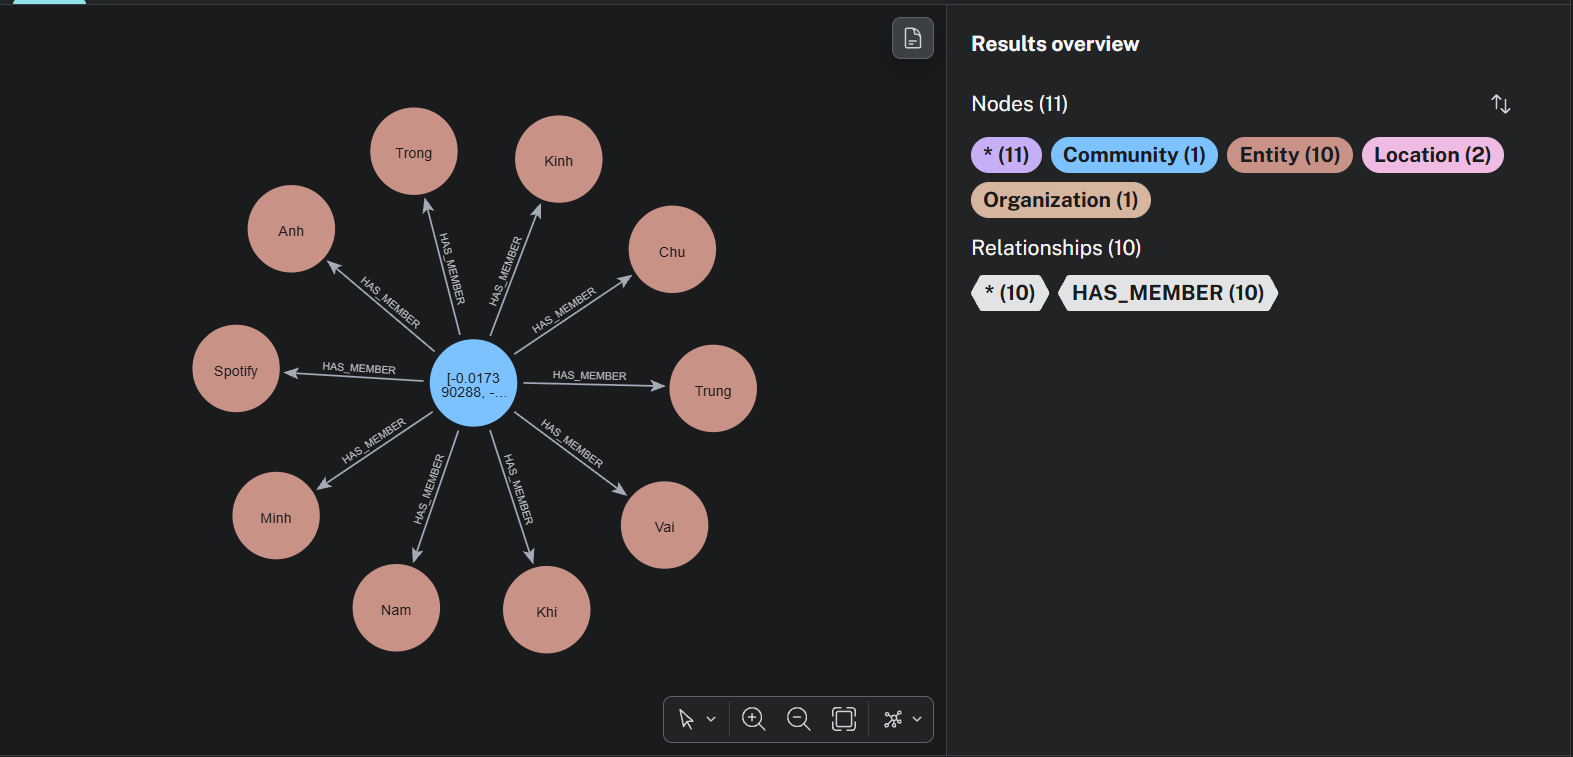
\includegraphics[width=\textwidth,height=0.62\textheight,keepaspectratio]{neo4j-screen/anh4.png}
\column{0.39\textwidth}
\begin{block}{Community layer}
\begin{itemize}
\item \texttt{Community -[:HAS\_MEMBER]-> Entity}
\item Communities summarize clusters of related entities and pages.
\item This layer helps the retrieval system surface broader thematic evidence.
\end{itemize}
\end{block}
\end{columns}
\end{frame}

\begin{frame}[shrink=8]{Algorithm Complexity and Design Rationale}
\begin{tabular}{p{.24\textwidth}p{.28\textwidth}p{.36\textwidth}}
\toprule
Technique & Role & Why it remained in the final system \\
\midrule
WRRF & Rank fusion & Robustly combines heterogeneous retrieval channels \\
Graph traversal & Evidence chaining & Improves multi-hop support coverage \\
Cross-encoder reranking & Candidate ordering & Lifts MRR after fusion \\
Agent routing & Question handling & Separates simple and complex reasoning paths \\
\bottomrule
\end{tabular}
\end{frame}

\begin{frame}{Weighted Reciprocal Rank Fusion}
\begin{block}{Fusion score}
\[
S_{\mathrm{WRRF}}(d)=\sum_{i\in\{b,v,g,c\}}\mathbb{I}[d\in L_i]\frac{w_i}{k+r_i(d)}, \qquad k=60.
\]
\end{block}
\begin{columns}[T]
\column{.48\textwidth}
\begin{itemize}
\item Fuses rankings rather than incompatible raw scores.
\item Deduplicates candidates by \texttt{chunk\_id}.
\end{itemize}
\column{.48\textwidth}
\begin{itemize}
\item Cross-encoder reranks the fused candidates.
\item Link expansion supports multi-hop evidence chains.
\end{itemize}
\end{columns}
\end{frame}

\begin{frame}{Evaluation Protocol}
\begin{columns}[T]
\column{.49\textwidth}
\begin{block}{Three settings}
\begin{enumerate}
\item Gold-context QA
\item Open-corpus retrieval
\item End-to-end QA
\end{enumerate}
\end{block}
\column{.49\textwidth}
\begin{block}{Metrics}
Hit@5, MRR, support recall, complete-chain recall, EM, F1, joint F1, abstention accuracy, and latency.
\end{block}
\end{columns}
\vspace{.35cm}
\begin{itemize}
\item Same ordered 240-item test set, graph snapshot, models, and seeds 42, 43, and 44.
\end{itemize}
\end{frame}

\begin{frame}{Final Retrieval Results}
\scriptsize
\centering
\begin{tabular}{lrrrrr}
\toprule
Method & Hit@5 & MRR & Support recall & Chain recall & Latency \\
\midrule
BM25 & 0.552 & 0.351 & 0.438 & 0.241 & 28.4 ms \\
Vector & 0.601 & 0.402 & 0.481 & 0.276 & 36.9 ms \\
Entity graph & 0.574 & 0.384 & 0.522 & 0.318 & 44.7 ms \\
WRRF & 0.684 & 0.472 & 0.603 & 0.391 & 63.8 ms \\
WRRF + reranking & \best{0.711} & \best{0.501} & \best{0.628} & \best{0.417} & 118.6 ms \\
\bottomrule
\end{tabular}
\vspace{.45cm}
\normalsize Fusion provides the strongest evidence coverage; reranking improves ordering at a measurable latency cost.
\end{frame}

\begin{frame}{Ablation Study}
\small
\centering
\begin{tabular}{lrrrr}
\toprule
Mode & Hit@5 & $\Delta$ Hit@5 & MRR & Mean latency \\
\midrule
Full hybrid & \best{0.711} & -- & \best{0.501} & 118.6 ms \\
Text only & 0.552 & -0.159 & 0.351 & 28.4 ms \\
Graph only & 0.574 & -0.137 & 0.384 & 44.7 ms \\
No reranking & 0.684 & -0.027 & 0.472 & 63.8 ms \\
No multi-hop & 0.648 & -0.063 & 0.443 & 92.1 ms \\
\bottomrule
\end{tabular}
\vspace{.45cm}
\begin{itemize}
\item Link expansion contributes 0.063 Hit@5.
\item Reranking contributes 0.029 MRR while adding 54.8 ms.
\end{itemize}
\end{frame}

\begin{frame}{End-to-End QA and Answerability}
\small
\centering
\begin{tabular}{lrrrrrr}
\toprule
Group & Answer EM & Answer F1 & Support EM & Support F1 & Joint F1 & Abstention \\
\midrule
All & 0.592 & 0.683 & 0.529 & 0.667 & 0.602 & 0.792 \\
Answerable & 0.521 & 0.653 & 0.443 & 0.641 & 0.536 & -- \\
Unanswerable & -- & -- & 0.726 & 0.726 & -- & 0.753 \\
\bottomrule
\end{tabular}
\vspace{.4cm}
\normalsize The remaining gap between retrieval and joint F1 motivates evidence-aware answer generation and abstention.
\end{frame}

\begin{frame}{Error Analysis and Limitations}
\begin{columns}[T]
\column{.49\textwidth}
\begin{alertblock}{Observed failure sources}
\begin{itemize}
\item Incomplete evidence chains
\item Entity-resolution noise
\item Unsupported answer synthesis
\item Incorrect abstention
\end{itemize}
\end{alertblock}
\column{.49\textwidth}
\begin{block}{System boundaries}
\begin{itemize}
\item Segment-to-chunk alignment remains incomplete.
\item NER noise can distort graph neighborhoods.
\item Aster chat is live; some visual fixtures are static.
\end{itemize}
\end{block}
\end{columns}
\end{frame}

\begin{frame}{Contributions}
\begin{enumerate}
\item A reproducible Vietnamese Wikipedia corpus pipeline with stable, verifiable evidence identities.
\item ViWikiHop: 1,600 answerable and unanswerable multi-hop QA records with group-aware splits.
\item Neo4j GraphRAG combining lexical, vector, graph, and community retrieval through WRRF.
\item Support-aware evaluation showing the benefit and latency trade-off of reranking and multi-hop expansion.
\end{enumerate}
\end{frame}

\begin{frame}{Conclusion}
\begin{block}{Main result}
The full GraphRAG configuration achieves \best{0.711 Hit@5}, \best{0.501 MRR}, and \best{0.417 complete-chain recall} on the ViWikiHop test set.
\end{block}
\begin{itemize}
\item Hybrid fusion is stronger than individual retrieval channels.
\item Link expansion and reranking improve quality, with explicit latency trade-offs.
\item Canonical evidence makes multi-hop results inspectable rather than answer-only.
\end{itemize}
\end{frame}

\begin{frame}[plain]
\centering
\vfill
{\color{fptNavy}\LARGE\bfseries Thank You}\par\vspace{.3cm}
{\large Questions \& Answers}
\vfill
\end{frame}

\end{document}
